While the inference servers discussed so far have exclusively utilized GPU resources, servers are easily portable and can run on other processing platforms. Previous uses of SONIC with FPGAs will be briefly summarized. In the new studies reported here, we have additionally run the Mini-AOD workflow with servers using both CPUs and Graphcore Intelligence Processing Units (IPUs)~\cite{Graphcore}.

\subsection{FPGAs}

The SONIC approach was first used with FPGA coprocessors to accelerate ML algorithms~\cite{Duarte:2019fta}. In this application, the ResNet-50 convolutional neural network~\cite{ResNet50} was retrained as a top quark jet tagger and as a neutrino event classifier. These algorithms were then hosted on the Microsoft Brainwave service~\cite{Brainwave}. It was shown that IaaS enabled per-inference latency reductions by a factor of more than 30, even including overhead and data transfer time between client jobs at Fermilab in Illinois and the Microsoft data center in Virginia. The SONIC client used for these studies relied on the construction of a server through Microsoft Brainwave. The Brainwave setup provided an end-to-end server framework that enabled the deployment of FPGA-based deep learning models to a gRPC server using a simplified gRPC protocol that differs from Triton, but remains compatible with SONIC. 

A second server implementation was developed, which relied on the Triton server protocols. This server, known as the FPGAs-as-a-Service Toolkit (FaaST)~\cite{FaaST}, was created to utilize several varieties of FPGAs and to add flexibility in the construction of the FPGA backend. The FaaST toolkit provides a framework for FPGA deep learning algorithm deployment using the same Triton protocol that serves as the default protocol for SONIC. Furthermore, this server setup was demonstrated to work both with local FPGA devices and in the cloud using Amazon Web Services. In this study, ResNet-50 was again accelerated for top quark tagging, as well as a small fully-connected neural network for HCAL local reconstruction. This algorithm was custom configured for the FPGA using the HLS4ML FPGA ML framework~\cite{Duarte:2018ite}. This was the first concrete demonstration of the portability of the SONIC approach; both the coprocessor technology and the server backend were changed without modifying the client-side code. Lastly, FPGA support can lead to optimized accelerator usage. Optimized FPGA inference can be achieved through the use of quantized neural networks, which can reduce the network overhead and improve the overall algorithm throughput. 

\subsection{CPU fallback server}
\label{sec:fallback}
%As discussed in Section~\ref{sec:sonic_benefits}, SONIC can factorize the ML software frameworks out of the client. Therefore, SONIC can be used as the default approach for inference even on local CPUs, eliminating the need to integrate third-party direct ML inference framework support into the experiment software (CMSSW). In addition, w
When running with remote servers, one potentially common and important failure mode is communication errors between clients and servers. In order to support automatic local CPU inference as a backup option when communication failures occur with remote servers, the SONIC implementation includes a service that can launch a Triton server using local CPU resources for any SONIC-compatible models, referred to as a ``fallback server''. Fallback servers can also be used for inference when third-party ML frameworks are not supported yet for direct inference. 

Ideally, the use of fallback servers should have minimal impact on per-event throughput relative to running direct-inference jobs without SONIC. This is contingent on two factors. Firstly, the latency introduced by sending data to/from local servers must be negligible. Secondly, servers should introduce minimal overhead in order to consume as few CPU resources as possible beyond what is needed to perform inference. The first concern can be resolved using the shared-memory option, which skips the gRPC communications and directly pass between servers and clients the data in a certain memory chunk. In reality, the gRPC overhead in most cases is found to be negligible. For the second concern, since local servers are running on the same CPUs as the other modules in the workflow, scheduling should be placed to avoid CPU thread contention between the two. This implies synchronous mode is preferred for local CPU fallback servers. Inference tasks should not create extra threads to avoid contentions. In the experiments we have found that more inference threads than the CMSSW job threads will slow processings down dramatically.

After some exploration, for the local CPU inference we run in synchronous mode, with the number of model instances set to the number of threads per job, and number of inference thread always 1. This way it can mimic the direct inference and avoid thread over-subscriptions as much as possible. We compare the throughput between direct inference and SONIC with local CPU servers with such configurations. Tests were performed using resources at the Purdue Tier-2 cluster with the CPU-only nodes. There are $n_{\text{CPU}}=20$ Intel E5-2660 CPU cores on one node, and hyperthreading is disabled to ensure more stable results. For all tests, the CPU nodes are always saturated by having the product of the number of jobs ($n_j$) and number of threads per job ($n_T$) to be the number of CPU cores: $n_j\times n_T = n_{\text{CPU}} = 20$. We scan the throughput as a function of the number of threads, as shown in Fig.~\ref{fig:throughput_cpu}. After optimizations, the throughputs of running on the local CPU fallback server are very similar to direct inference now. The higher throughputs in some cases are due to more recent versions of ONNX inference version installed inside the server, which can be controlled in the real productions.

\begin{figure}
    \centering
    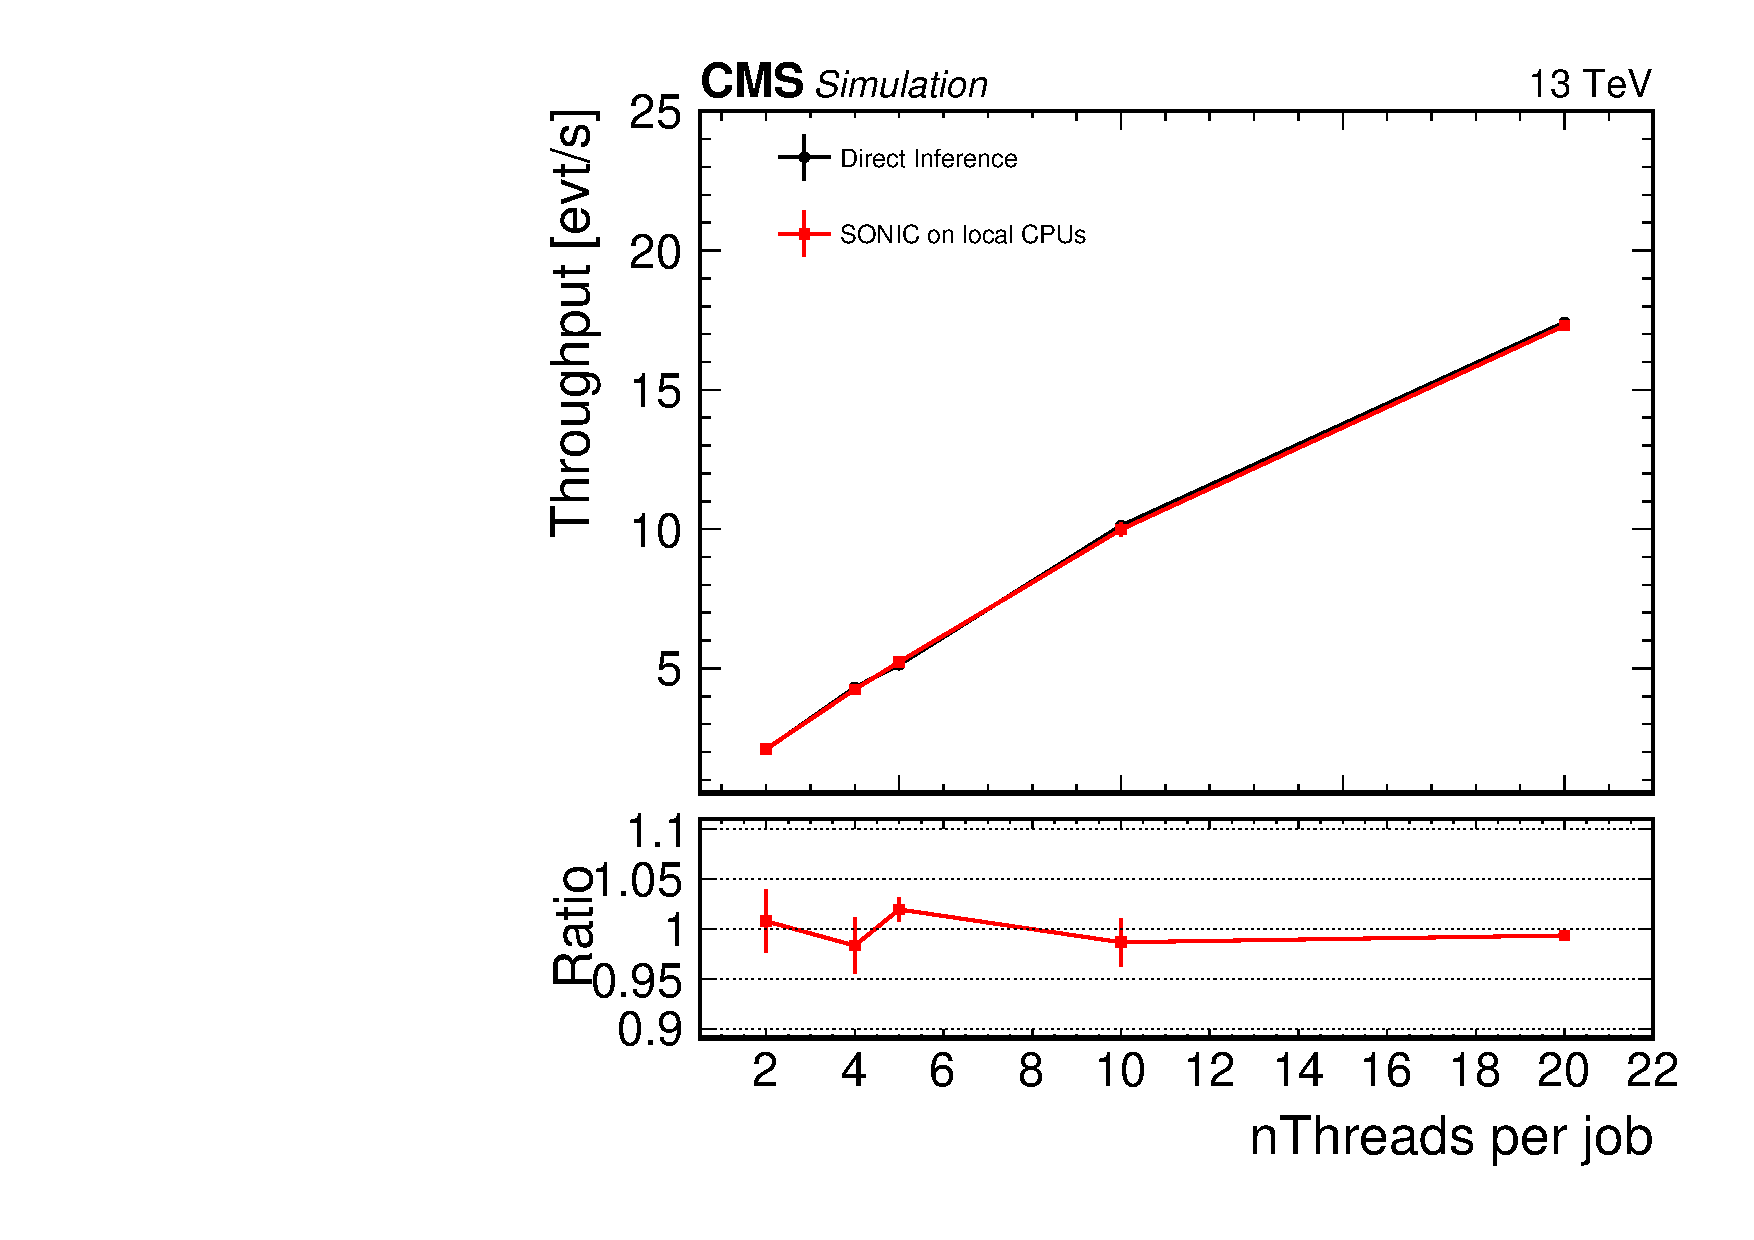
\includegraphics[width=0.50\textwidth]{plots/CPUTest_throughput.pdf}
    \caption{Throughput (top) and throughput ratios (bottom) between SONIC and direct inference in the local CPU tests at Purdue Tier-2 Cluster. In order to ensure the CPUs are always saturated, in all the tests the number of threads per job multiplied by the number of jobs is set to 20.}
    \label{fig:throughput_cpu}
\end{figure}


\subsection{Studies with Graphcore IPUs}
\textcolor{red}{Detailed contents are in discussion with GraphCore team.}

As discussed in Sections~\ref{sec:triton} and~\ref{sec:sonic_benefits}, NVIDIA Triton inference servers support custom backends to run with different coprocessors and different (ML) backends. Since the SONIC client code only depends on the Triton protocols, algorithms implemented in this way can easily be ported to different types of coprocessors. One of the Mini-AOD production tests was done together with the GraphCore IPU team, where they prepared a custom backend to support running ML inference with IPUs. The current supported ML frameworks include \TENSORFLOW and \PYTORCH, with \ONNX and \PYTORCHGEOMETRIC support in development. This allows us to run DeepMET and DeepTauID inference on IPUs. Without any modifications on the client side, we reconfigure the workflow configuration to point the clients to IPU servers on the Graphcloud cluster, and successfully run DeepMET and DeepTauID models via SONIC, while running the other parts of the Mini-AOD workflow on local CPUs.
